\chapter{Introduction}
\label{ch:introduction}

\todo{Versuchen ein universelles Beispiel zu finden, dass sich durchzieht}
\todo{gesamtes Dokument: Trennen Algorithm vs. Method}

\textit{Anomaly Detection (AD)} has been around since we started collecting data. Early scientists relied on simple observations and charts to look for anything abnormal. For instance, in the 16th century, astronomers like Tycho Brahe observed the night sky with high precision, recording unusual celestial events. When Brahe observed a supernova, it marked a significant anomaly in his records that contradicted the belief, the night sky would not change and propelled advancements in astronomy \cite{Decourchelle2017}.

Today, we can leverage additional tools, like statistics, \textit{Machine Learning (ML)} and \textit{Artificial Intelligence (AI)} to enhance our ability to detect anomalies. These technologies allow us to analyze much bigger amounts of data, revealing patterns and insights that would have been hidden to the naked eye.

As we reflect on the journey of AD from the precise charts of Brahe to the powerful algorithms today, it becomes clear that detecting and understanding anomalies is not just about identifying outliers. It is about discovering the abnormal in our data and learning from it, ultimately driving innovation across various fields.

In this master thesis, we want to continue this journey by providing insights into the vast variety of AD techniques. Past research has shown that the great diversity of patterns still asks for the careful eye of researchers to thoughtfully apply the right technique to their data. Just like Brahe, modern scientists need to carefully analyze their data and have a deep understanding of the tools they use. We want to support this process by mapping existing techniques from different fields to emerging patterns in time series data to provide guidelines for picking the appropriate tool.

To achieve this and contribute to this journey, we start by delivering the foundations for understanding the dataset. We introduce the characteristics and specialties of time series data and explain common modeling techniques. We further define anomalies and categorize them so the analyst know what to expect. The last brick of the foundation is the explanation of AD techniques. In this section, a taxonomy is introduced to categorize the different approaches and develop an overview. Before we introduce the current state of the art from the literature, we discuss the problem this master thesis is dealing with and define what is in- and outside its scope. 

The literature review introduces decomposition and feature extraction on time series data before jumping to a thorough analysis of AD algorithms. The comprehensive review of different approaches towards AD, their strengths and weaknesses forms a great part of the added value of this paper to the journey of AD

%\section{Background and Motivation}
% why good to detect anomalies
%The goal of this master thesis is to provide guidelines to the readers, so they can make an informed decision on which algorithm suits their use-case. As mentioned above, different algorithms have different strengths and weaknesses depending on the given data characteristics. For instance, deep learning algorithms with \textit{Long-Short-Term Memory (LSTM)} can capture patterns across many time steps, while . Such incorporated structures must be understood to map them to the expected anomalies. But, to perform such a mapping, a deep dive into the different types of anomalies is essential to understand their diversity, which is often much more complex than breaking a simple threshold. Within the scope of this work, the discussed data structure in which the anomalies appear are time-series. So in order to conclude the path towards the final guidelines, we start by understanding these special data structures.

\section{Time Series}
\label{sec:time_series}
\todo{einigen auf "time series data"/ "time series"/ "time-series"}
% Introduction to time series
A time series is a sequence of data points recorded at discrete time during specific intervals. The data points are often real numbers, which are typically spaced uniformly. The primary characteristic that distinguishes time series data from other types of sequential data is the temporal order, which is extremely common when observing real world phenomena \cite{Cryer2009}. 

We follow a general definition of time series \cite{Kreis2006}:
\begin{equation}
    \label{eq:time_series}
    X = (X_t : t \in T), \quad T = \mathbb{Z},
\end{equation}

Where $t$ denotes the time index and $X_t$ are real-numbered data points, which can be multidimensional $X_t \in \mathbb{R}^n$. We further note that $T = \mathbb{N}$ is another common definition of time series as it usually starts at a specific point in time (e.g. $t=1$). However, $T=\mathbb{Z}$ assumes an infinite past and does not require special treatment of an initial value.

% univariate, equidistant
In Equation \ref{eq:time_series} we assume that the time series is \textit{equidistant}. This means that the data points $X_t$ were collected at regular, uniformly spaced intervals. This regularity simplifies the analysis, as many time series models assume equidistant intervals for their mathematical formulations \cite{Chatfield2003}.
Non-equidistant time series are rare but can occur in domains like healthcare, where patient visits may not follow a regular schedule. Analyzing non-equidistant time series often requires specialized techniques that can handle the irregular spacing of data points.
Formally, if the time series is equidistant, then for all $t$ and $t'$ where $t \neq t'$, the time intervals $\Delta t = t_{k+1} - t_k$ are constant.

The formulation in Equation \ref{eq:time_series} can also describe one-dimensional data points $X_t \in \mathbb{R}$, which makes $X$ a \textit{univariate} time series. In the multidimensional case above, it is called \textit{multivariate}.
Univariate time series record one variable at a time, such as a stock price \cite{Sinha2022}. Multivariate time series, on the other hand, record multiple variables simultaneously, which can be of the same type or a mixture of different data types \cite{Chandola2009}. For example in economics, analysts might consider variables like GDP, inflation, and commodity price together \cite{Verstyuk2019}.
In the field of AD, univariate time series can often be handled by simpler models as they are less computationally expensive, while multivariate models can capture the interdependencies between variables, offering a more comprehensive understanding of a system \cite{Chandola2009}.

To complete the justification of using Equation \ref{eq:time_series} as our definition of time series, it should be mentioned that there are also continuous time series definitions. However, the concept of continuous time series comes into play in a theoretical or modeling context. Since this work deals with observations recorded at distinct, separate time points, Equation \ref{eq:time_series} for discrete time series is considered adequate.

\subsection{Real-World Examples}
% - Where are time series coming from
Time series are ubiquitous and can be found across various domains, like finance, meteorology or healthcare. 
In finance, stock prices are one of the most common examples. They are recorded at regular intervals, such as daily or minute-by-minute, and are used to analyze market trends and make investment decisions. 
In meteorology, temperature readings taken at regular intervals (e.g., hourly) form a time series that can be analyzed to understand weather patterns, climate change, and seasonal variations. 
In healthcare, heart rate monitoring involves recording heart rates at regular intervals, often in real-time, to monitor a patient’s health condition and manage chronic diseases. 
In each of these examples, the overall goal is to analyze patterns, detect anomalies or forecast future values based on the recorded time series data. A significant aspect of \textit{time series analysis (TSA)}.


\subsection{Analysis and Characteristics}

\begin{figure}
    \centering
    
\includegraphics[width=0.5\linewidth]{images/placeholder.png}
    \caption{Run Chart of a Time Series}
    \label{fig:run_chart_example}
\end{figure}

% - characteristics of time series
In real world applications, such as the examples given above, time series are often captured over longer periods of time, which leads to long sequences. The straight forward approach is to plot such sequences in a run chart, like in Figure \ref{fig:run_chart_example}, to get meaningful insights into the data. With longer sequences, however, it can be difficult to discover patterns within the plot. The goal of TSA is to use the right techniques to describe past patterns to detect, eliminate or forecast past and future patterns \cite{Vishwas2020}. 

Someone could easily imagine how this could be translated to AD. In fact, AD is a subset of TSA, which uses its techniques to model a normal behavior and distinguish the unusual. For this reason, this section only covers the time series characteristics derived from TSA as modeling is covered in Chapter \nameref{ch:literature_review}.

Understanding the different characteristics within time series is essential for an effective analysis. Generally, time series can be analysed in the \textit{time domain} or the \textit{frequency domain}, which are not mutually exclusive \cite{Shumway2017}.
The time domain approach covers the temporal dynamics of the data, such as the relationship between current values and past values. It excels in understanding direct temporal relationships and forecasting.
The frequency domain approach covers the cyclical behavior in the data. Instead of looking at how past values influence future ones, it examines the series in terms of periodic cycles or oscillations. It is particularly useful for detecting regularities and periodicities that might not be obvious in the time domain.
Generally speaking, while the time domain is concerned with "when" changes happen, the frequency domain is focused on "how often" changes happen.

Shumway and Stoffer \cite{Shumway2017} formulated a set of time series characteristics around these domains using real experimental data:

% Wichtig weil kommt zur Sprache in def. anomaly
\paragraph{Temporal correlation} is one of the primary characteristics of time series data, meaning that an observation $X_(t')$ can be highly dependent on its previous observations where $t<t'$. This poses a challenge for traditional statistical methods, which often assume independence among observations \cite{Student1908, PEARSON1920, Fisher1992, Russell2020, Edgeworth}. However, in certain contexts, the \textit{Markov property} can be applied, suggesting that the future state of a process depends only on its present state and not on its past states. This simplifies the analysis by allowing models to focus on the most recent observations. Measures such as \textit{autocovariance} or \textit{autocorrelation} (explained in \ref{}) help models to account for temporal correlations by capturing the dynamic nature of the data while following the Markov property when appropriate.

\begin{figure}
    \centering
    % First Row of Subfigures
    \begin{subfigure}[b]{0.45\textwidth}
        \centering
        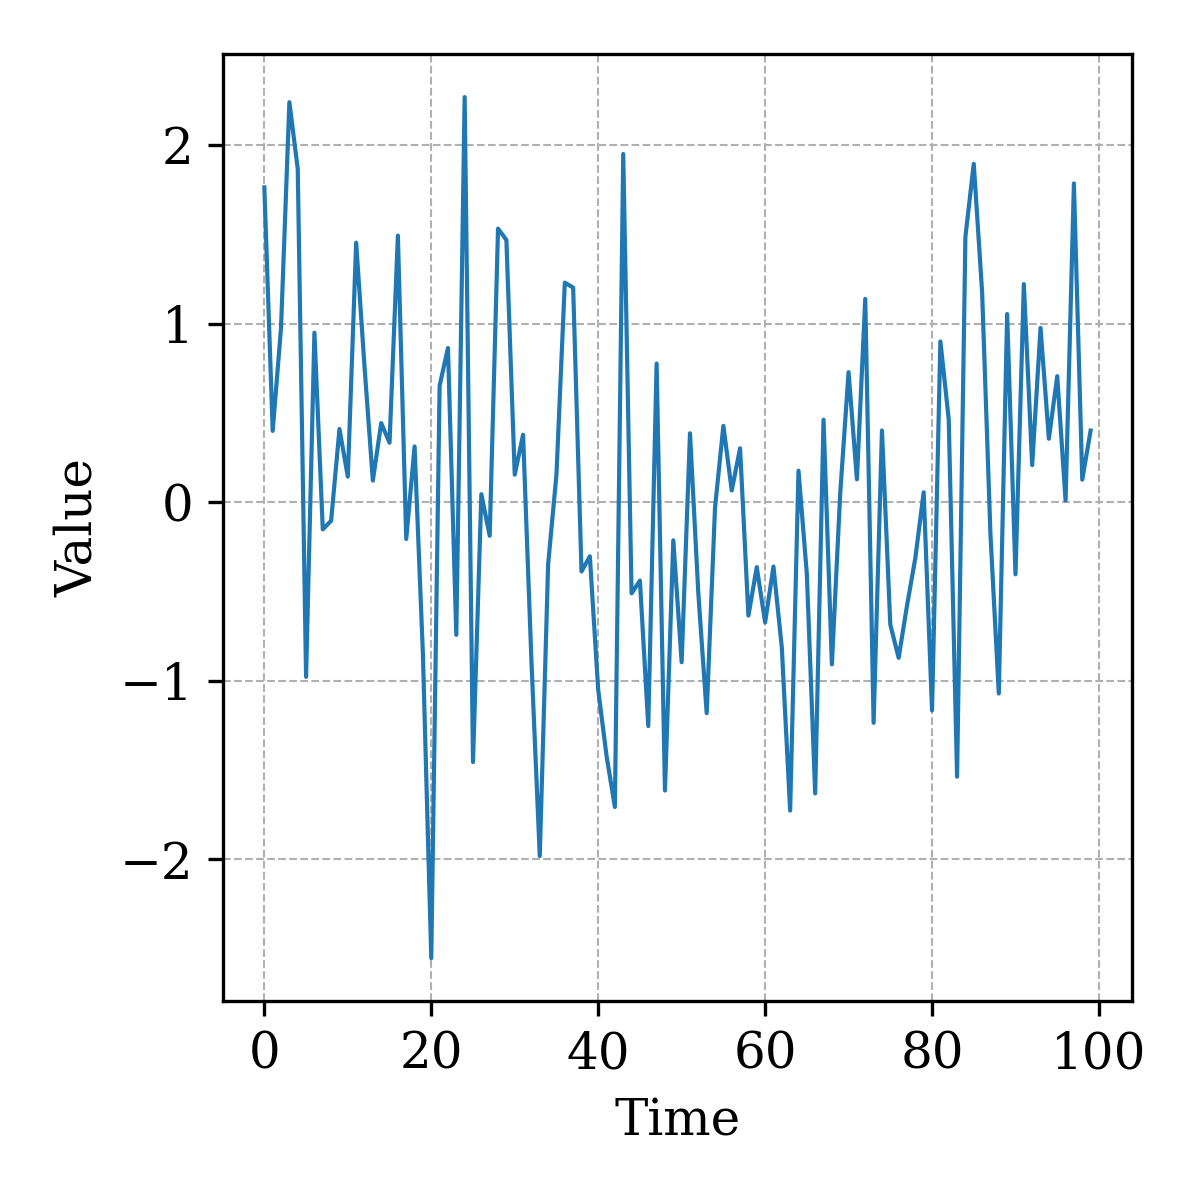
\includegraphics[width=\textwidth]{plots/stationarity_plots/stationary_time_series.png}
        \subcaption{Stationary Time Series}
        \label{fig:stationary}
    \end{subfigure}
    \hfill
    \begin{subfigure}[b]{0.45\textwidth}
        \centering
        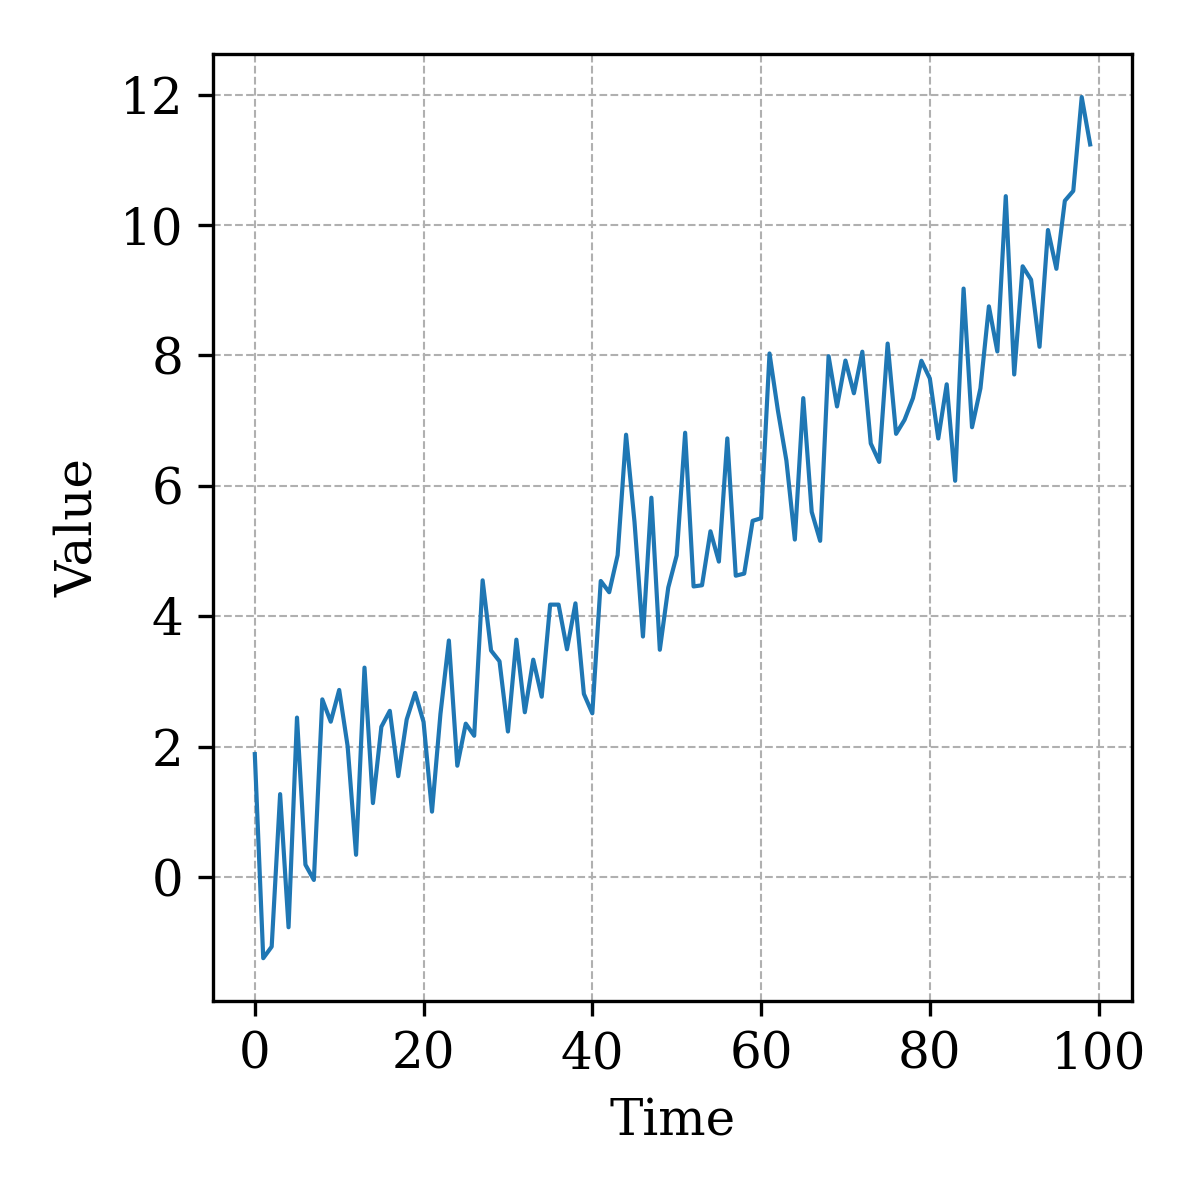
\includegraphics[width=\textwidth]{plots/stationarity_plots/nonstationary_time_dependent_mean.png}
        \subcaption{Non-Stationary Series with Time-Dependent Mean}
        \label{fig:nonstationary_mean}
    \end{subfigure}
    % Second Row of Subfigures
    \vskip\baselineskip
    \begin{subfigure}[b]{0.45\textwidth}
        \centering
        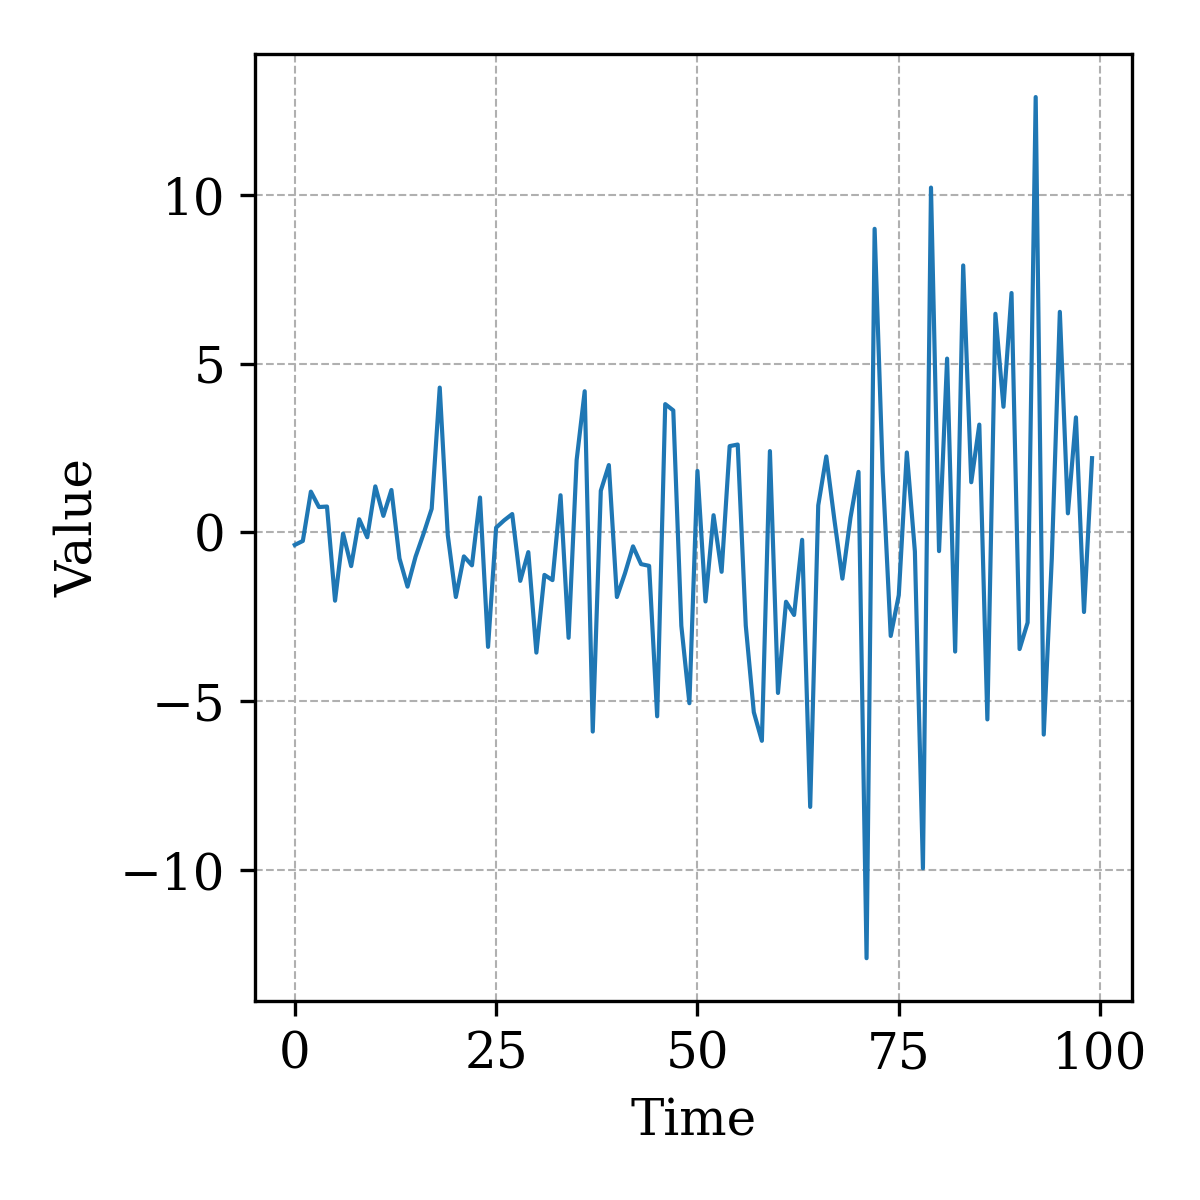
\includegraphics[width=\textwidth]{plots/stationarity_plots/nonstationary_time_dependent_variance.png}
        \subcaption{Non-Stationary Series with Time-Dependent Variance}
        \label{fig:nonstationary_variance}
    \end{subfigure}
    \hfill
    \begin{subfigure}[b]{0.45\textwidth}
        \centering
        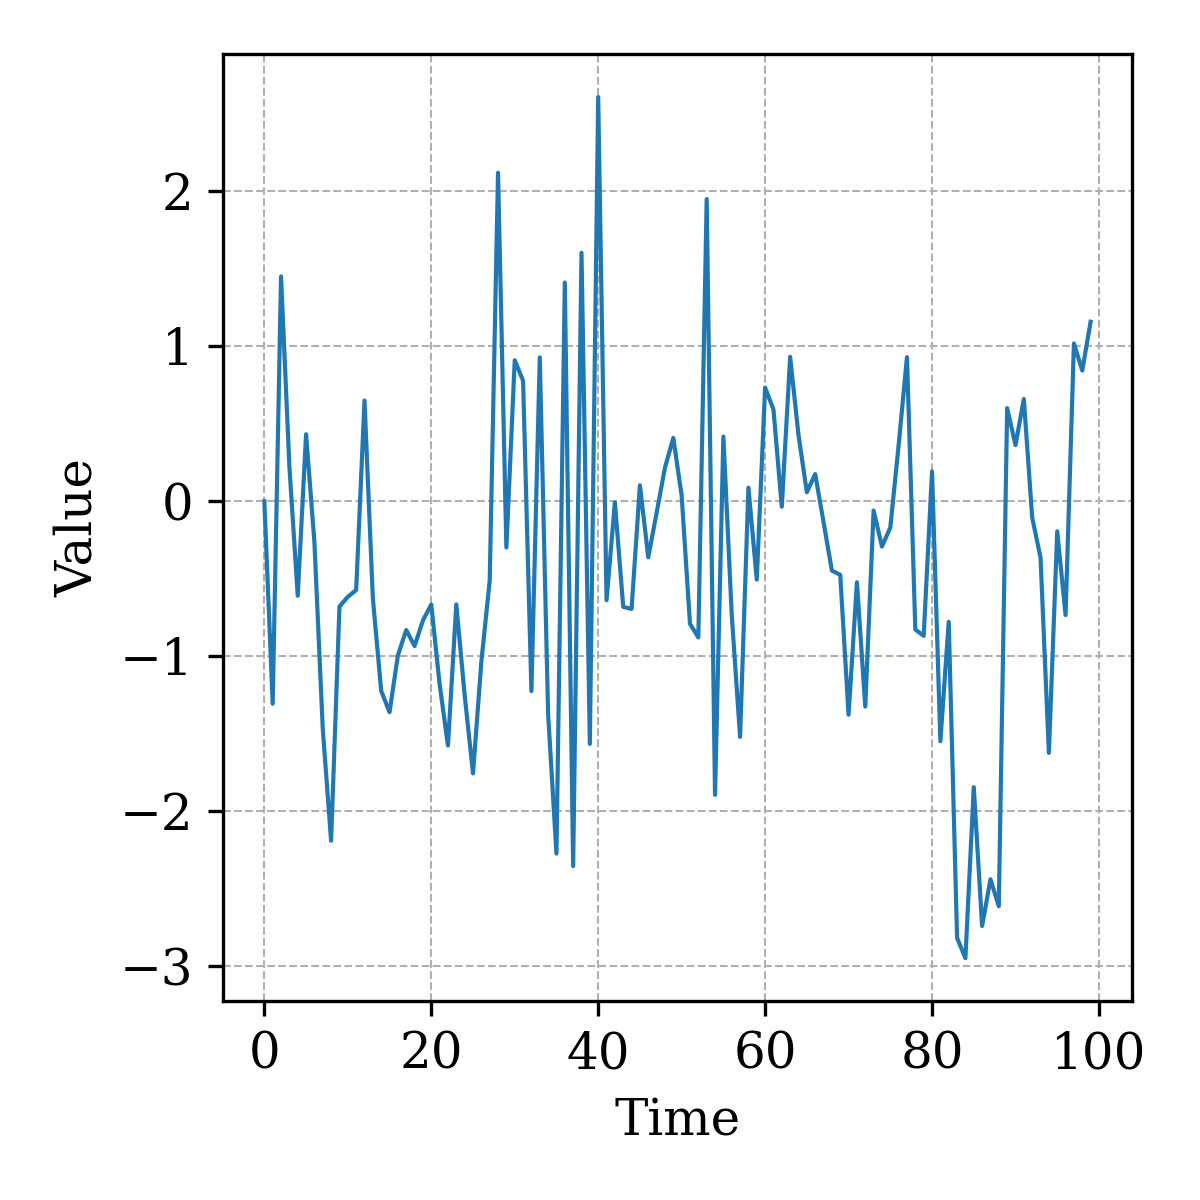
\includegraphics[width=\textwidth]{plots/stationarity_plots/nonstationary_time_dependent_covariance.png}
        \subcaption{Non-Stationary Series with Time-Dependent Covariance}
        \label{fig:nonstationary_covariance}
    \end{subfigure}
    \caption{Comparison of Stationarity and Non-Stationarity in Time Series}
    \label{fig:stationarity_comparison}
\end{figure}

\paragraph{Stationarity} refers to a characteristic where statistical properties such as mean and variance remain constant over time, like in Figure \ref{fig:stationary}. 
However, time series can show trend, seasonality or cyclic components, which introduce non-stationarity. The key concept is to perform a transformation and achive stationarity, as non-stationary data can lead to misleading statistical inferences and poor forecasting performance \cite{Hamilton1989}. 

A \textit{trend ($T$)} refers to a long-term movement, indicating an overall increase or decrease in the data over an extended period. It is usually represented by the mean rate of change over time and, therefore, is a type of non-stationarity \cite{Vishwas2020}. In Figure \ref{fig:nonstationary_mean} we illustrated a linear, upward trend, which shows in the graph and is indicated by a linearly increasing mean. Generally, a trend pattern can also be nonlinear, which makes its identification difficult.

\textit{Seasonal ($S$)} and \textit{Cyclic ($C$)} components involve fluctuations, rather than long-term movements. Seasonalities are regular patterns with a fixed and predictable duration, like a temperature increase and decrease during the day. Cyclic patterns, in contrast, are not as regular or predictable, like economic cycles. Both patterns can introduce all three types of non-stationarities from Figure \ref{fig:stationarity_comparison} to different degrees. Differentiating between the two is crucial to transform the non-stationarities accordingly \cite{Box2013}. 

\paragraph{Irregularities ($I$)} are unexpected variations or random noise within the data. They appear irregularly but usually do not effect stationarity.

We take Equation \ref{eq:time_series} and \textit{decompose} the time series $X_t$ at any time $t$ to a linear (Equation \ref{eq:linear-decomposition}) and non-linear (Equation \ref{eq:non-linear-decomposition}) model of its components \cite{Vishwas2020}:

\begin{equation}
\label{eq:linear-decomposition}
    X_t = T_t + S_t + C_t + I_t
\end{equation}
\begin{equation}
\label{eq:non-linear-decomposition}
    X_t = T_t \cdot S_t \cdot C_t \cdot I_t
\end{equation}

After decomposing the time series using such a model, each component can be tackled individually to achieve stationarity. 


\section{Anomalies}
% - What are anomalies: explain anomaly; anomaly vs. outlier; anomaly detection KURZ erklären
We introduced trend, seasonality and cycle patterns above. With the knowledge about their nature and by taking a look at the Figure \ref{fig:stationarity_comparison} again, the sudden changes already appear anomalous. But are these patterns already \textit{anomalies}?

In the field of anomalies in time series, defining an anomaly is both crucial and complex. An anomaly, in a general contexts, is something that deviates significantly from the norm, raising suspicions about its origin or nature \cite{mw:anomaly}. This definition can be put into the context of statistics. Here, data points that are far from the distribution are considered \textit{outliers}. However, it is difficult to determine how far a data point needs to deviate from the distribution in order to be considered an anomaly. Hawkins \cite{Hawkins1980} refines this by saying that an outlier has to deviate to such an extend that it was caused by a different mechanism other than random error in order to be an anomaly. 

This definition is very close to the terms \textit{abnormal} \cite{cb:abnormal} or \textit{deviant} \cite{cb:deviant}, which is why they are often used interchangeably \cite{Whitehead1995}. In this work we use the term \textit{anomaly} exclusively to avoid confusion. In the literature review in Chapter \ref{ch:literature_review}, other terms might appear, which are used by the authors of the presented paper. This helps to link the information to the origin paper but it is always made clear that it is a synonym of "anomaly".

In some contexts, \textit{novelty} \cite{cb:novelty} is used as a synonym for anomaly. However, in the field of AD it is important to differentiate between the two terms. For instance, a smart watch user lends his device to a friend. Due to novel arm movements, the smart watch detects them as anomalies and the watch stops working properly. This example shows how novelties need to be distinguished from anomalies to become part of the system's normal behavior, which is often not trivial.
\todo{Einbauen: anomaly = imbalanced datasets per definition}

Going back to the initial question, we now answer that the time series follows a normal behavior and significant deviations are considered anomalies. Decomposition describes the normal behavior in a more refined way and offers better comparison to define the anomalous.  

\begin{figure}
    \centering
    \begin{subfigure}[b]{0.45\textwidth}
        \centering
        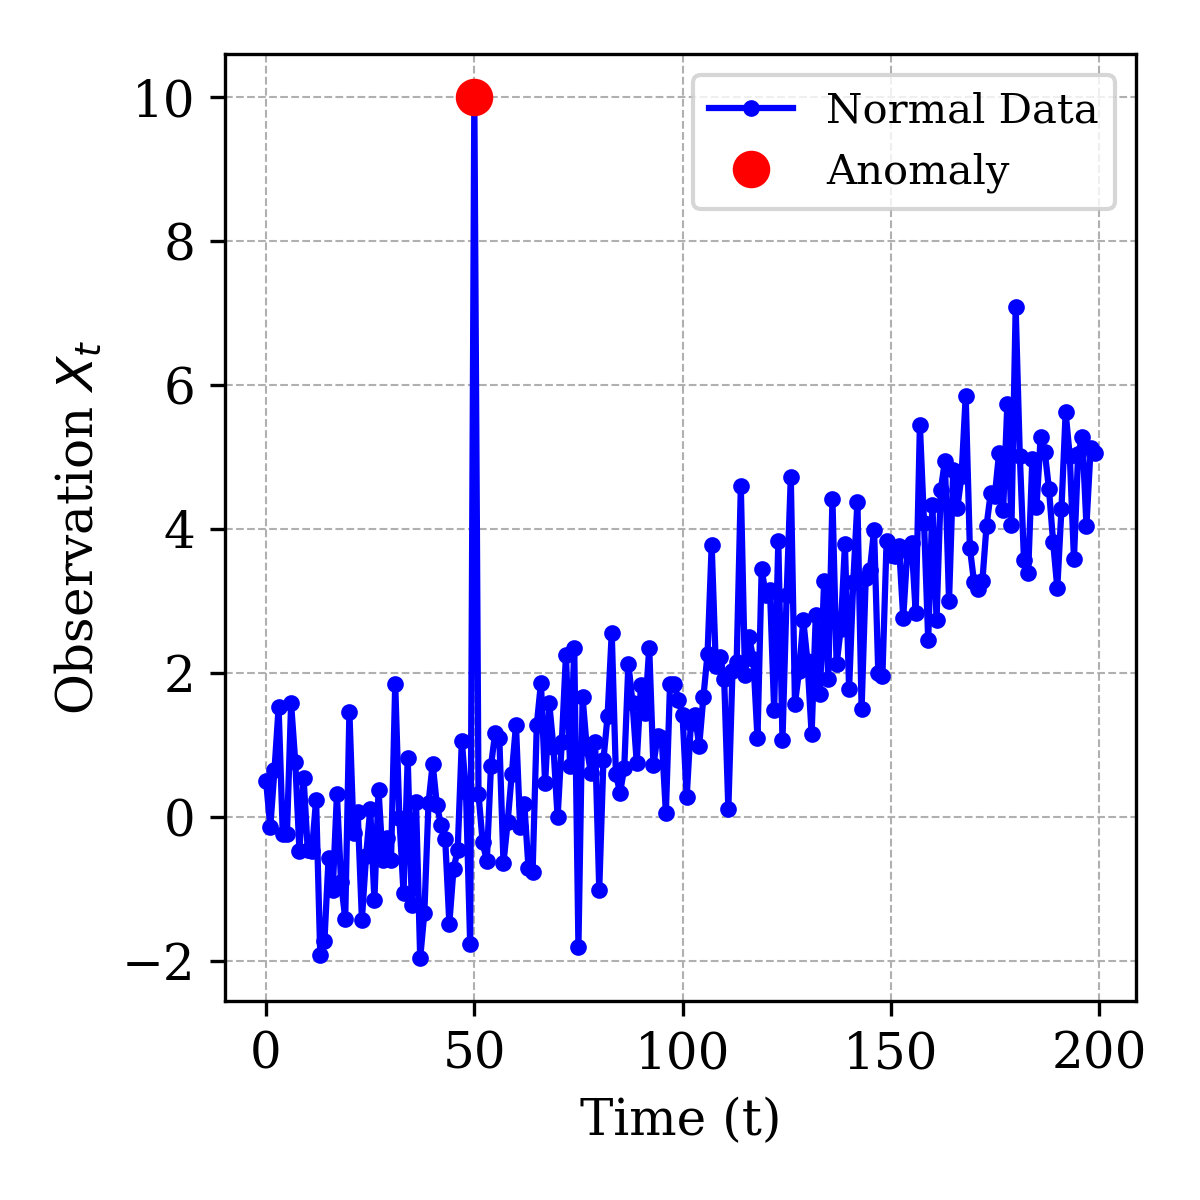
\includegraphics[width=\textwidth]{plots/temporal_correlation_plots/run_chart_with_anomaly.png}
        \subcaption{Run Chart of $X$}
        \label{fig:run_chart}
    \end{subfigure}
    \hfill
    \begin{subfigure}[b]{0.45\textwidth}
        \centering
        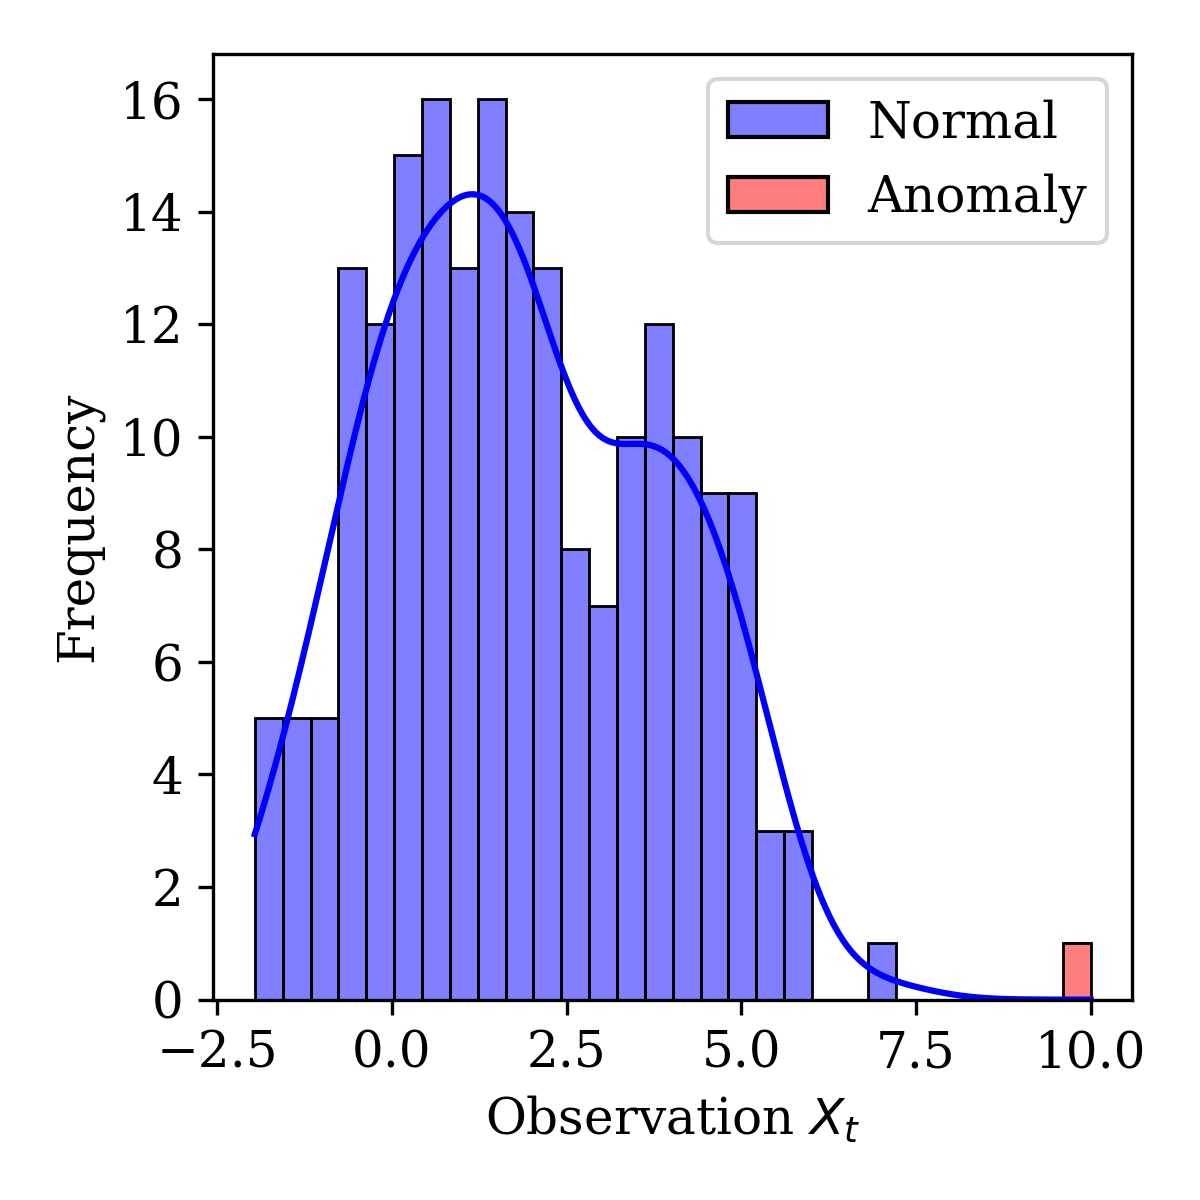
\includegraphics[width=\textwidth]{plots/temporal_correlation_plots/distribution_chart_with_anomaly.png}
        \subcaption{Distribution of all $X_t \in X$}
        \label{fig:distribution_chart}
    \end{subfigure}
    
    \caption{Time Series with Extremum and Trend Anomaly}
    \label{fig:temporal_correlation_comparison}
\end{figure}
Anomalies in time series data also differ from other data types, where it might sorely depend on the underlying statistical properties and distributions. We observe Figure \ref{fig:run_chart}, where the data points $X_t$ are plotted along a time axis in sequential order $X$. We notice a spike around $t=50$, which clearly strikes as an anomaly. We also observe a following upward trend, which is not visible for $t<50$ and should also be considered anomalous. If we observe Figure \ref{fig:distribution_chart}, where we neglected the temporal order by plotting the distribution of all $X_t$, we can detect the anomaly $X_{50} = 10$ as it is outside the distribution. However, the distribution does not show the trend anomaly as it simply caused it to skew. 

This example shows that the importance of respecting the temporal correlation when detecting anomalies in time series. It also shows that there are different types of anomalies. Chandola et al. \cite{Chandola2009} formulates three anomaly types:

\begin{itemize}
    \item \textit{Point anomalies} are data instances, which significantly differ from the rest of the data, like the anomalous data point $X_{50}$.
    \item \textit{Contextual anomalies} are only considered anomalous in a specific context but may appear normal otherwise, like the trend anomaly for $t>50$. These anomalies require the definition of a context as an overall trend could also be considered a component of the time series' normal behavior. 
    \item \textit{Collective anomalies} are groups of related data instances, which appear anomalous relative to the entire dataset, even if some instances do not appear anomalous. For example, a consistent sequence of low values in an electrocardiogram reading could signify a heart condition, even though individual low readings may be normal.
\end{itemize}

Contextual and collective anomalies show that the AD is no trivial task. We highlight the importance of defining the normal behavior to improve the detection of the abnormal. We introduced the concepts of modeling and decomposing time series to better understand and transform the normal behavior. Using this refined definition of our normal behavior, we can use a more typification of anomalies by introducing nine \textit{anomaly kinds} \cite{Schmidl2022}:

\begin{itemize}
    \item \textit{Amplitude Anomalies} occur when one or multiple consecutive values deviate significantly in magnitude from the norm. This type of anomaly is characterized by spikes or drops that stand out from the typical range of values. They indicate potential errors, sudden changes in conditions, or unexpected events.

    \item \textit{Extremum Anomalies} refer to data points that represent extreme single values, either as unusually high peaks or low troughs within the data. These anomalies can signify exceptional events, such as system overloads, failures, or extreme external conditions affecting the data. The peak $X_50$ in Figure \ref{fig:run_chart} could be considered an extremum anomaly.

    \item \textit{Frequency Anomalies} involve fluctuations in the periodicity of the data. They occur when there is a change in the frequency of a known recurring event. This highlights the importance of analysis of the frequency domain for AD.

    \item \textit{Mean Anomalies} characterized by deviations from the expected average value of the time series. A mean anomaly indicates a shift in the central tendency, such as long-term drifts or gradual changes.

    \item \textit{Pattern Anomalies} are deviations in the sequence or structure of data points that disrupt the normal pattern. These anomalies reflect unexpected changes in the order or combination of events.

    \item \textit{Pattern Shift Anomalies} represent shifts in the position of a known pattern within the time series. Unlike pattern anomalies, pattern shift anomalies maintain the integrity of the pattern but occur at unexpected times.

    \item \textit{Platform Anomalies} involve deviations from a stable baseline or platform level. Such anomalies suggest that the data has shifted away from a consistent state, which may signal phase changes, structural breaks, or other fundamental shifts in the baseline behavior of the system.

    \item \textit{Trend Anomalies} occur when there is a change in the direction, slope, or rate of progression of the trend component $T$.

    \item \textit{Variance Anomalies} involve changes in the variability or dispersion of the data points around the expected value. An increase in variance may indicate rising instability or volatility, while a decrease may suggest a reduction in expected fluctuations.
\end{itemize}

\todo{visualize all anomaly kinds?}

%\subsection{Anomaly Detection Techniques}

\section{Problem Statement}
% Generalization
In classification problems a tight fit is important in order minimize bias and improve accuracy, but, it is often secondary to the models capability to generalize well. 

This is also the case for AD problems. Peterson et al. \cite{Peterson2007} emphasize the importance of good generalization. On the one hand, a tight fit can complicate the differentiation between novelties and anomalies, leading to many false alarms. On the other hand, such models can overlook anomalies that resemble normal instances as they usually have to classify data points that do not conform to any learned classes. For instance, attackers that try to infiltrate a companies intranet with spam e-mails try to mimic normal e-mail traffic. However, their attacks should have some nuance differences, which the model must catch while avoiding sending many harmless e-mails to the spam folder.

In the context of time series data a good generalization translates into a good representation of the underlying dynamic structures. However, this poses a greater challenge for AD in time series than in other domains.

A model with a well balance between tight fit and generalization introduces components, like trends, as part of the normal behavior, while not overly relying on them.

As explained earlier, such components are context dependent, like a trend that can be an anomalous sensor drift or a seasonal temperature increase. This shows that the differentiation of anomalies and evolving patterns might depend on complex temporal dependencies. Many researchers tried to deal with the complexity of a given dataset by estimating the dependencies and tailoring a matching algorithm, which led to a great existence of algorithms from various families. Each of these approach has its strengths and weaknesses but often lag the described balance between tight fit and generalization. In addition, the literature lags a set of guidelines, estimating good performing algorithms based on given data characteristics. This is crucial, as the literature already shows that the variety of dependencies can not be modeled by one approach alone \cite{Schmidl2022}.   
   
% Objectives
In this work we want to tackle the complexity of anomalies in time series by refining the classification of anomalies using a categorization proposed by Schmidl et al. \cite{Schmidl2022}. The idea is to use the refined categorization to split the complexity of anomalies and tackle each one individually based on their special characteristics. By setting algorithm families and refined anomaly categories against each other, we aim to identify structural benefits of the different algorithms. Linking these benefits with different anomalies provides a mapping from expected anomaly dependencies to potential best-performing algorithms.

\section{Scope and Limitations}
% Only univariate
This research focuses on the anomaly detection techniques specifically within the context of univariate time-series. This decision is driven by the simpler and more controlled environment, the observation of a single variable offers. By leveraging this control, we aim for robust and interpretable results, which could be adapted to more complex systems. Additionally, it further increases practicality as many researchers struggle with multivariate data and more complex models \cite{Chandola2009}. 
However, there are inherent limitations to this focus. By concentrating on univariate data, the research does not directly address the challenges associated with multivariate time series. 
While the findings of this study are expected to contribute to the understanding of anomaly detection in simple cases, they may not fully capture the complexities and interdependencies of multivariate scenarios. 

% Only unsupervised
This research further excludes data labels entirely, which would be leveraged by supervised or semi-supervised approaches. We argue that a sheer focus on unsupervised data provides a more flexible and scalable framework, especially in anomaly detection where labeling data is challenging. Therefore, this study aims for contributions, which are not limited by the availability of labeled data.
It is important to note that this limitation can enhance usability but does not address the potential benefits of labeled data. Additional labels provide clear guidance for model training, which could improve detection precision and reduce false positives. While the findings of this study are expected to advance the understanding of unsupervised anomaly detection, they may not fully leverage the insights that could be gained from labeled data.

% Thesis Structure